\section{Frameworks and Processes in RE}
Es gibt keinen idealen RE Prozess. RE beinhaltet zwei Hauptschritte
\begin{itemize}
	\item R Spezifikation\\
	Elicitation\\
	Analyse\\
	Dokumentation\\
	Validierung
	
	\item R Management\\
	Release Management\\
	Modification, Change Management\\
	Verfolgbarkeit
\end{itemize}

Ein paar relevante Aspekte in RE Prozessen
\begin{itemize}
	\item linear oder inkrementell\\
	\textit{Linear:} R sind eindeutig/klar; geringes Risiko; Kurze Entwicklungszeit\\
	\textit{Inkrementell:} R nicht offensichtlich; hohes Risiko; lange Entwicklungszeit
	\item Rolle des Spezifikationsdokumentes (Vertrag? Müssen R von Dritten impl. werden?)
	\item Mglkeit des teilnehmenden Ansatzes (inkludieren des Kunden)?
	\item Produkt für speziellen Kunden oder Markt?
\end{itemize}

\textbf{Mögliche Process Patter}
\begin{itemize}
	\item \textbf{Vorschreibend}
	\begin{itemize}
		\item alle R müssen erfüllt werden
		\item Projektziele wichtiger als Deadlines und Kosten
		\item SRS als Vertrag 
		\item oft linearer Dev-Prozess
		\item oft Arbeit mit Dritten
	\end{itemize}
	
	\item \textbf{Explorativ}
	\begin{itemize}
		\item R müssen innerhalb eines Menge von globalen Projektzielen erarbeitet werden
		\item Kunde/Nutzer aktiv in Prozess eingebunden
		\item R priorisiert
		\item oft Deadlines/Kosten wichtiger als Erreichen der Ziele
		\item in der Regel inkrementell
	\end{itemize}
	
	\item \textbf{Reactive}
	\begin{itemize}
		\item System mit Standardsoftware impl
		\item R müssen an diese Std-Software adaptiert werden
		\item R oft nicht ins Detail ausgearbeitet
	\end{itemize}
	
	
	\item \textbf{Kundenspezifisch}
	\begin{itemize}
		\item initiiert durch Kundenauftrag
		\item Stakeholder können identifiziert werden
		\item Stakeholder auf Kundenseite sind Hauptquellen für R
	\end{itemize}
	
	\item \textbf{Marktorientiert}
	\begin{itemize}
		\item Kunden und potenzielle Nutzer sind schwer zu identifizieren
		\item R meist von Devs spezifiziert; Devs müssen quasi Bedürfnisse der Kunden erahnen
	\end{itemize}
\end{itemize}

\textbf{Typische RE-Prozesse} können durch eine Kombination von Patterns beschrieben werden
\begin{itemize}
	\item \textbf{Vertrag}\\
	oft linear; vorschreibend; Kundenspezifisch
	
	\item \textbf{teilnehmender Ansatz}\\
	inkrementell; explorativ; kundenspezifisch
	
	\item \textbf{Productorientiert}\\
	inkrementell; oft explorativ; marktorientiert
	
	\item \textbf{Nutzen von Standardsoftware}\\
	linear od inkrementell; reactive; kundenspezifisch
\end{itemize}

\subsection{User-centered Approach}
interaktive Software sollte sein: \textbf{nützlich, nutzbar} und \textbf{used}(=brauchbar oder benötigt?!)\\
User-Centered Design erfordert:
\begin{itemize}
	\item früher Fokus auf User, Aufgaben und Umfeld
	\item aktive Einbringung des Users
	\item angemessene Zuordnung von Funktionen zw User und System
	\item Einarbeitung von User-Feedback in das System
	\item iterativer Entwurfsprozess mit Entwurf, Testen und Modifizieren von Prototypen
\end{itemize}

\begin{figure}[!h]
	\centering
	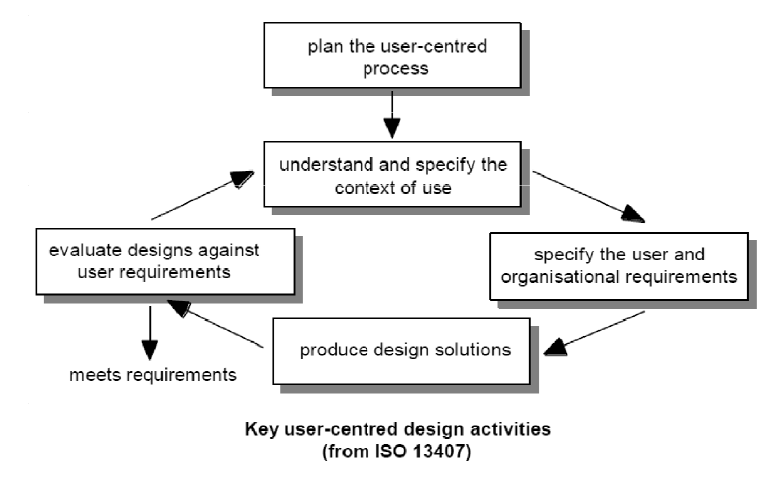
\includegraphics[scale=0.7]{img/user_centered_activities.png}
	\caption{User-centered Design Activities}
\end{figure}


\begin{figure}[!h]
	\centering
	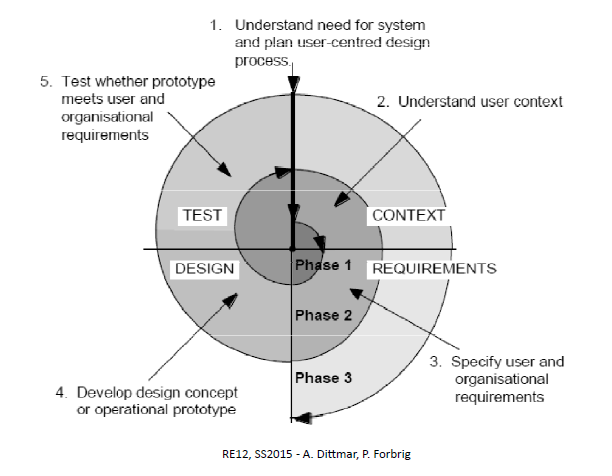
\includegraphics[scale=0.7]{img/user_centered_activities_app2.png}
	\caption{User-Centered Design - R and design cycle}
\end{figure}


\newpage
\section{Prototyping}
- Prototyp = konkreter, aber nur teilhafte Darstellung oder Implementierung eines Systems\\
- verschiedene Techniken; Gemeinsamkeit = alle machen abstrakte Ideen lebendig\\
- interaktiv\\
- nützlich, weil Kunde kann sich eine Vorstellung vom System machen, mit Prototypen arbeiten

\subsection{Throw Away Prototype}
\begin{itemize}
	\item entwickelt für initiale R, aber nicht genutzt fürs finale Projekt
	\item geschriebene Spezifikation der R
	\item einige Devs glauben dies ist Zeitverschwendung
	\item easy to use Sprache
\end{itemize}

\subsection{Evolutionary Prototype}
\begin{itemize}
	\item fundamentalste Form des Prototyping
	\item Hauptkonzept: Robusten Prototypen entwickeln und stetig verbessern
	\item Ziel: User ein funktionierendes System liefern
\end{itemize}

\begin{table}[!h]
	\centering
	\begin{tabular}{|p{20em}|p{20em}|}
		\hline
		\textbf{Pros}	& \textbf{Cons}\\
		\hline
		ständig nach neuen Wegen zur Systemverbesserung suchen & benutzbar um Dokumentation der R zu vermeiden\\
		\hline
		erhöhte Chance Kunden zufrieden zustellen & Management wird vor.\\
		\hline
		kann benutzt werden, wenn R nicht def. sind & Long Term Wartung kann teuer sein\\
		\hline
		schnellere Auslieferung des Systems & unklare Entwurfsideen\\
		\hline
		& Informationsverlust durch viele Verbesserungen/Iterationen\\
		\hline
	\end{tabular}
	\caption{Pros \& Cons of evolutionary prototyping}
\end{table}

\subsection{Lo-Fi Prototyping}
\begin{itemize}
	\item Prototyp mit eingeschränkter Funktion, Interaktion
	\item Demonstriert allgemeines Look and Feel; stellt Konzepte, Alternativen und einfach Screen Layouts dar
	\item entwickelt zum Zeigen, Kommunizieren, Inspirieren; nicht als konkrete Basis zum Implementieren gedacht
	\item am Anfang des Entwicklungszyklus benutzt um allgemeine Konzepte zu zeigen; ohne viel Zeit in Entwicklung zu investieren
	\item Beispiel: Paper-Prototype
\end{itemize}

\subsection{Hi-Fi Prototyping}
\begin{itemize}
	\item stellt Kernfeatures/Kernfunktionen des UI dar
	\item voll interaktive Systeme; User kann Daten eingeben, erhält Rückmeldungen etc; kann damit interagieren und arbeiten
	\item Trade-Off: Speed <-> Genauigkeit
	\item hohe(r) Kosten und Ressourcenverbrauch
\end{itemize}

\subsection{Summary}
\begin{table}[!h]
	\centering
	\begin{tabular}{|p{20em}|p{20em}|}
		\hline
		\textbf{Pros}	& \textbf{Cons}\\
		\hline
		Stakeholder können Möglichkeiten und Einschränkungen des Systems besser verstehen & schwer alternative Prototypen zu evaluieren\\
		\hline
		User-Centered Lösungen (betreffend das UI) & Bewertung der Stakeholder können widersprüchlich sein\\
		\hline
		Kommunikation zw User, Dev, Analyst etc & quick and dirty development\\
		\hline
		Stakeholder können einfacher neue Ideen vorschlagen & komplexe Probleme sind schwer darzustellen\\
		\hline
	\end{tabular}
\end{table}
